\chapter{Beyond V1: Variance and Thalamo-Cortical Loops}

\begin{flushright}
    \textit{''Welcome back my friends \\
    to the show that never ends. \\
    We’re so glad you could attend, \\
    Come inside! Come inside!''}\\
    Emerson, Lake and Palmer, Karn Evil 9, 1973
\end{flushright}

\chaptertoc{}

\section{Introduction: The Functional Anatomy of the Pulvinar}
After having had the pleasure of immersing ourselves in more than a hundred of pages of \gls{V1}-centric research, it now seems only natural to take a break away from the striate cortex. As alluded to in the thesis's introduction, \gls{V1} takes part in parallel computations distributed both in extrastriate regions and in subcortical nuclei. These interactions are crucial for inverse variance processing, and now call for our attention for a proper description of a "multiscale" computational system. One particularly intriguing facet of these interactions is the role that the pulvinar nucleus plays. This thalamic nucleus operates as a sophisticated "routing" system, modulating the information flow between \gls{V1} and extrastriate regions~\cite{casanova2004functions}. Given the interest we took in the modulation of integration between multiple cortical regions by the inverse variance, the presence of a thalamic nucleus interconnected with this entire network is undeniably a brain region worthy of deeper exploration. 

Before detailing more the involvement of pulvinar in predictive coding, we shall briefly introduce its anatomy and functions. The first article of this chapter consists of a review of the role of pulvinar in this domain, aiming to introduce similar notions, and hence it would be redundant to go into too many details here. It should be noted that, in the context of this thesis, some theories suggest that the pulvinar might be the primary locus of inverse variance weighting in the brain~\cite{kanai2015cerebral}, while others suggest it only plays a part in this role~\cite{millidge2021predictive}.

Anatomically, the pulvinar lies over the dorsolateral posterior thalamus, running alongside the edge of the \gls{LGN}. In primates and in cats, the pulvinar is the largest thalamic nucleus, having increased in size throughout mammalian evolution with the visual cortex~\cite{hutchins1989retinotopic}. Given its size, the pulvinar can be further subdivided in six sub-regions in primates (human included) or three main regions in the cat~\cite{arcaro2015anatomical}, which, out of scope, will be here simplified as a single conceptual entity in this introduction (but see the first article for further details). The pulvinar establishes extensive reciprocal connections with all visual cortical areas~\cite{jones2012thalamus}, often being conceptualized as the "seventh cortical layer"~\cite{shipp2003functional}. In a striking difference with the \gls{LGN}, which receives its main visual inputs from the retina, the pulvinar receives its visual inputs principally from the layers 5 and 6 of the visual cortex. This is reflected in the response characteristics of its neurons, which remarkably resemble those found in the visual cortex in terms of feature selectivity~\cite{merabet1998motion}, but also in their implementation of selective attention~\cite{werner2004visual,villeneuve2012pattern}. This allows pulvinar neurons to effectively suppress responses to visual distractors~\cite{robinson1992pulvinar} by integrating the visual signals from multiple cortical areas and outputting modulatory signals to layers IV and I of the visual cortex. Overall, the pulvinar’s connectivity gives it an integrate-and-modulate role within the visual hierarchy. This description is especially relevant when considering the visual system as a hierarchical generative Bayesian model within the predictive coding framework (Equation~\ref{eq_pc_matrix}).

As put forward by Kanai et al.~\cite{kanai2015cerebral}, the pulvinar’s engagement in attentional regulation and its output connectivity to superficial cortical layers is an ideal match for a role in inverse variance modulation of the visual hierarchy, which also fits the long timescales of multi-areas integrations. Experimental results have shown that inactivation of the pulvinar drastically suppresses responses of superficial \gls{V1} neurons to sensory inputs, while excitation increases the responsiveness of neighbouring superficial units with overlapping receptive fields~\cite{purushothaman2012gating}, which is similar to a gain-control mechanism that implements inverse variance-weighted modulation of the cortex by the pulvinar. Whilst it is the biggest thalamic nucleus in primates, the pulvinar is nonetheless an order of magnitude smaller than the entire visual cortex. As estimating inverse variance requires computting the co-variance between the all $N$ prediction or prediction errors units, this is an $N^2$ computation~\cite{millidge2021predictive}. Given the cost of such computation, it seems more likely that the pulvinar computes an approximation of the inverse variance matrix, and then modulates parts of the superficial layers independently. In parallel, these units will then use their local horizontal connectivity to further integrate and refine the computation of the local variance~\cite{kanai2015cerebral, bastos2012canonical}, as proposed in chapter 4~\cite{ladret2023cortical}. Evolutionarily, this hypothesis is very interesting, as some species, such as birds, have much lower homologous "cortical" (i.e. pallium) neuron count, and seem to lack a functional equivalent of the pulvinar. In a thesis committee discussion with Dr. Paul Cisek, we hypothesized that as the number of neurons grow exponentially throughout evolution, computing variance through recurrence alone (as proposed in chapter 4), becomes either prohibitively slow or computationally expensive. This thus requires a dedicated central part of the neural network to perform a dynamical approximation of the inverse variance matrix, which would hence be the role assigned to the pulvinar.

\begin{figure}[h!tbp]
\vspace{0.1cm}
\centering
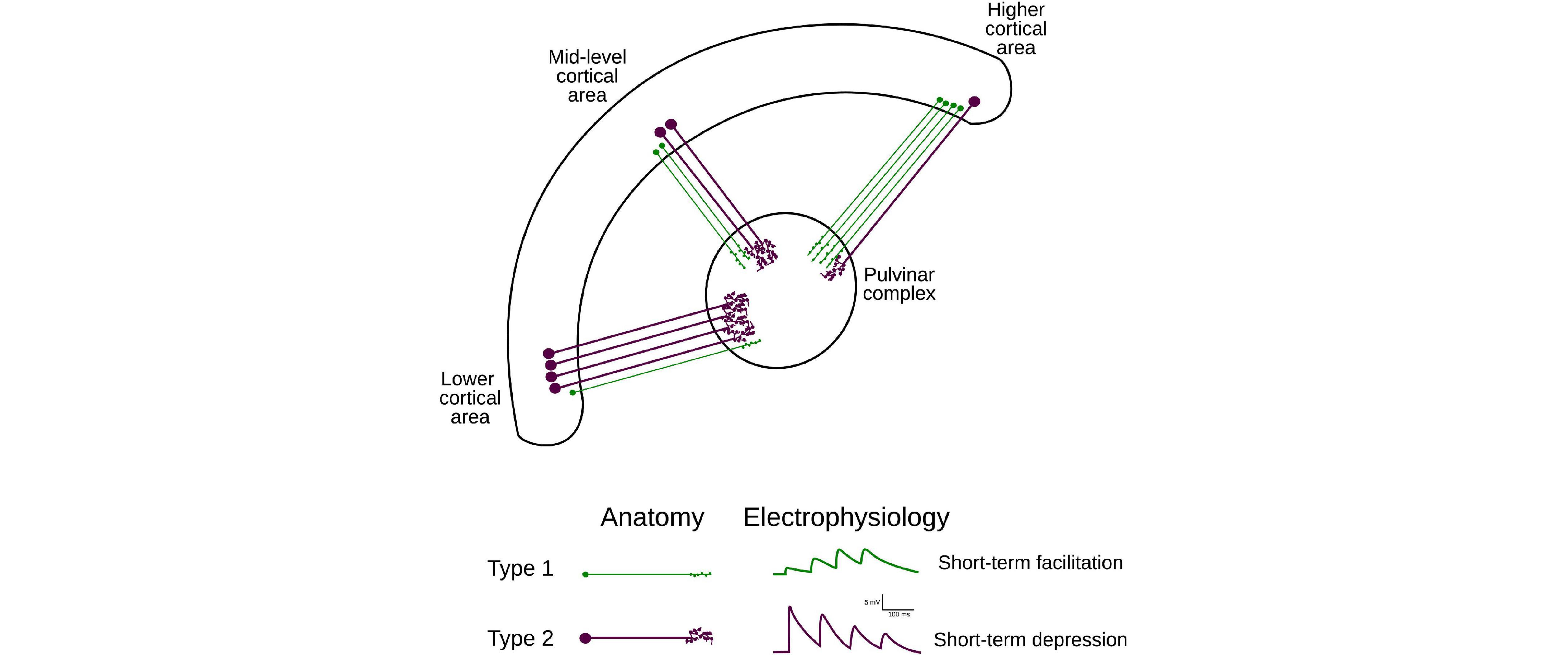
\includegraphics[width=1.\textwidth]{fig/chap7_gain_control.pdf}
\caption[Anatomical substrates of pulvinar gain control.]{Anatomical substrates of pulvinar gain control, from~\cite{cortes2021corticothalamic}. Note that the ratio of Type 1 over Type 2 synapses changes as a function of the visual hierarchy.}
\label{fig_chap7_gain_control}
\end{figure}

Overall, this depicts a dynamical gain control role for the pulvinar, much like the gain control role we proposed in chapter 4. How is such dynamical gain control in the visual cortical areas implemented ? Guillery and Sherman~\cite{guillery2002thalamus} characterized synapses associated to thalamic first-order relays, which transfer information about the world to primary cortical areas (in vision, the \gls{LGN}). Two types of inputs, modulators and drivers (type 1 and type 2 projections, respectively), have been identified on the basis of their axon terminals’ morphology and their electrophysiological characteristics~\cite{sherman1998actions}. Drivers and modulators can also be defined by other attributes, such as the input-output transfer of the neuronal response profile. Modulators effects are distinguished as either multiplicative or divisive effects (nonlinear gain control), while drivers act by either additive or subtractive changes (linear gain control)~\cite{abbott2005drivers, silver2010neuronal}. In \gls{V1}, it is generally accepted that pulvinar receives type II projections (confirmed driver signals) from layer 5 neurons and sends back anatomically defined type I projections (modulatory) to layer 1. In the case of higher-order cortical areas, the assumption is that pulvinar receives type I projections from layer 6 neurons (suspected modulators) and projects to layer 4 (suspected drivers) (Figure~\ref{fig_chap7_gain_control}. In the context of predictive coding, this functional distinction between drivers and modulators is crucial, as drivers are associated with predictions and modulators with precision. Precision may coordinate and broadcast more globally visual information and its regulation may be equivalent to selective attention~\cite{creutzfeldt1988extrageniculo}, which can be implemented by modulator connectivity from the pulvinar. This notion of driver and modulators will be discussed further in the first article of this chapter, which reviews additional functional evidences, but also in the second article, which models the heterogeneity of these two types cortico-thalamic pulvinar connections and their role on the propagation of prediction-related alpha oscillations. 

\section{Review: "The Pulvinar as a Hub of Visual Processing and Cortical Integration"}
This review for \textit{Trends in Neuroscience} aims to provide an overview of the hypothesized roles of the pulvinar. Given the extensive connectivity, one can find what they would like to find in this nucleus, and thus we aim to review the recent evidences for pulvinar in terms of attention, feature binding, predictive coding, and global workspace theory. 

Full citation is as follows: \fullcite{cortes2023pulvinar}

As this is a review rather than a research article, we direct the reader to Appendix B. There, they will find a comprehensive overview of the response properties of the pulvinar and their interpretation under predictive processing.



\section{Methods: Oscillations and Predictions}
As we discussed in the introduction and in the review, the pulvinar is involved in performing a gain control modulation onto \gls{V1}~\cite{purushothaman2012gating}. This can be conceptualized as a (predictive) gating mechanism, that can control the propagation of message passing from \gls{V1}. In the case of an overly high variance input, the pulvinar can thus "explain away" the activity of \gls{V1}, preventing an erroneous update of the internal brain models. But, in the opposite case, what is the influence of \gls{V1} on the pulvinar ? If, according to our article in chapter 4, \gls{V1} can compute the inverse variance of visual inputs, then it should be able to send that information in some form to the global regulator of the message passing to other cortical areas. Furthermore, if there is such a thing as this global regulator of inverse variance-weighting implemented the pulvinar~\cite{kanai2015cerebral}, then it is crucial to look at how \gls{V1} it interacts with the pulvinar, in that directed fashion. 

To understand the nature of this communication, we must first understand the nature of the message being sent. Disentangling sensory predictions from prediction errors is already arduous enough in \gls{V1} and we must turn our attention to another method to study inter-area communications. For that, it is better to study the propagation of activity from the cortex to the pulvinar in terms of frequency. This relies on the idea that, in predictive coding, one posits the existence of a single prediction error unit (not necessarily a neuron) for every prediction unit. As these units must be connected only to one another, and in the form of a negative feedback loop (see Equation~\ref{eq_pc_matrix}, predictive coding essentially implies a neural network that works as coupled oscillatory pairs of prediction errors and prediction units~\cite{friston2019waves}. The lowest characteristic frequency of this response, as determined empirically, lies in the alpha range ($8-12 \text{Hz}$), which is the dominant brain rhythm at rest, when prior models require no novel error updating. This also translates into many psychophysical-relevant peaks in response to a stimulus, as recorded in EEG (N1, P2, for example~\cite{bruyns2017neurogenesis}). 

\begin{figure}[h!tbp]
\centering
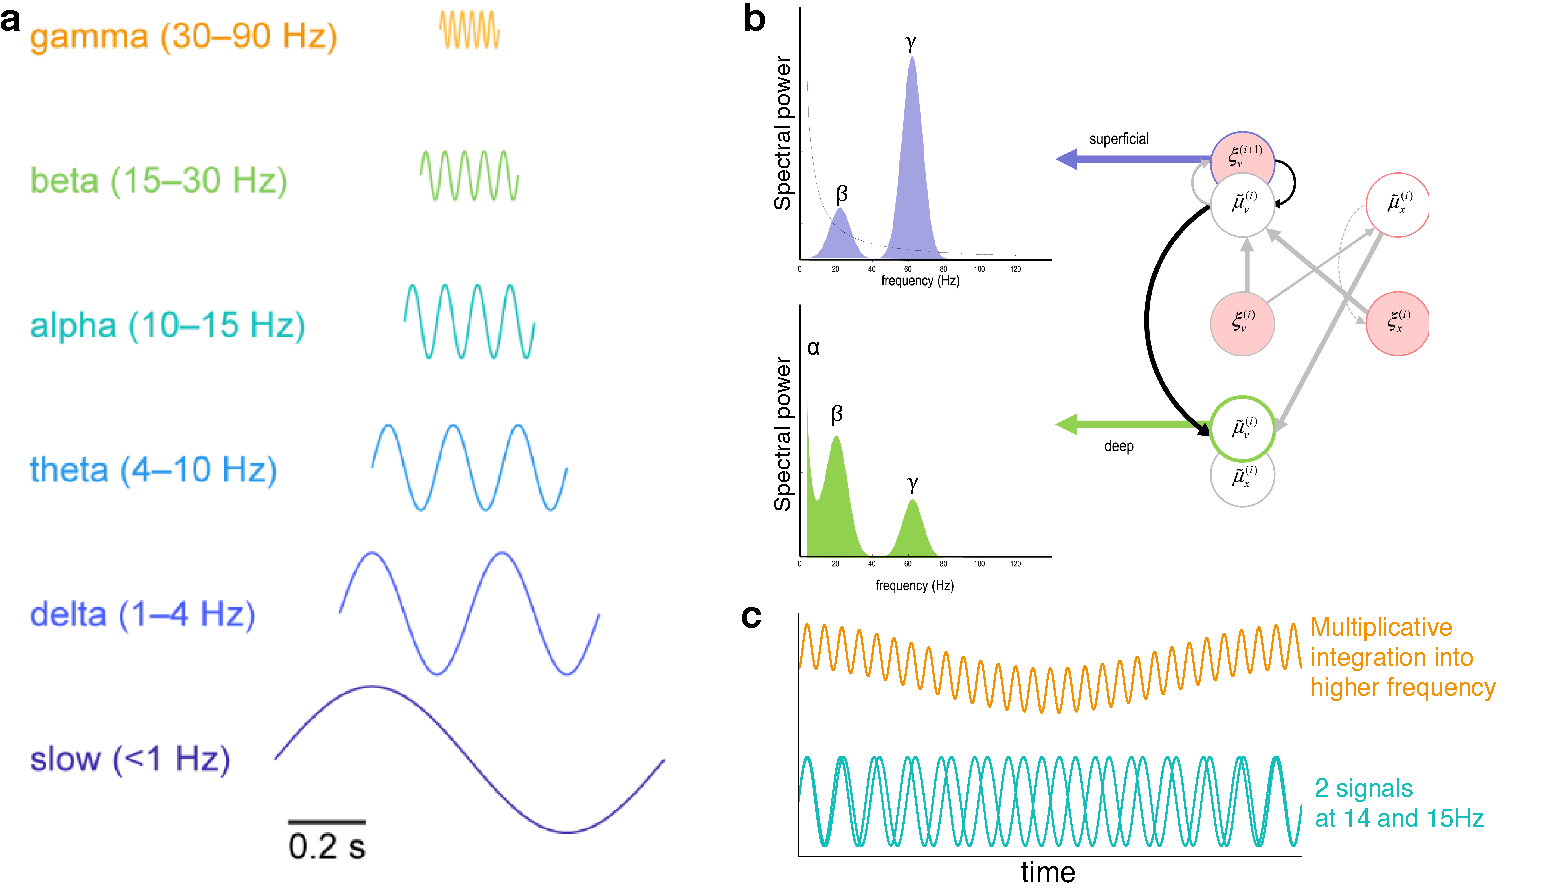
\includegraphics[width=1.\textwidth]{fig/fig_chap7_oscillations.pdf}
\caption[Neurobiological oscillations.]{Neurobiological oscillations and predictive coding. (a) Frequencies of oscillations found in neurobiological recordings. (b) Types of oscillations posited by a predictive coding neural network, from~\cite{bastos2012canonical}. (c) Illustration of the multiplication of two alpha-band predictive signals into a gamma-band prediction error.}
\label{fig_chap7_oscillations}
\end{figure}% oscillation figure + bastos frequencies + nonlinear mixtures (with the sine mixing)

The picture becomes more complex when one needs to understand that resolution of erroneous predictions through propagation of errors are not instantaneous. Predictions, fundamentally, should be based on the multimodal interactions of cortical areas, but also of multi-features interactions within a single modality. Practically, a prediction about a high-variance Motion Clouds is the interaction between multiple prediction error units, each signaling a single edge.

This means that the message passing in predictive coding occurs through a series of nonlinear transformation, implying that many alpha range signals will be transformed into higher frequency through this exchange. This summed interaction is often assigned to the second most prominent range of communication in the brain, gamma-band ($40 Hz$). Prediction errors, as they are based on this non-linear mixtures of expectations, must be present in those higher frequencies. Predictions, as they are more stable and need not be updated constantly (which forms the defining principle of predictive coding), should be only found in lower frequency. This "spectral asymmetry" of cortical communication~\cite{bastos2012canonical, bastos2015visual} explains many attentional mechanisms~\cite{kok2012attention}. This is also replicated with minimal assumption in silico, by showing that coupled neuronal oscillators with biological time constants, i.e. conduction delays of $12$ ms and synaptic time constant of $20$ ms naturally create an emergent alpha/gamma prediction/error oscillation.

It follows that spectral asymmetry also implies (functional) anatomical asymmetry, namely in the canonical model that predictions can be found in deep layers~\cite{bastos2012canonical}. Thus, given the anatomy of the corticothalamic projections, it would seem that predictions only are sent to the pulvinar. This effectively allows it to regulate which prediction of a given level of the visual hierarchy is best suited to provide the best explanation for an external sensory cause, based on its precision. This is specifically the theoretical principle we discuss in this article, by showing how alpha (predictive) rhythms in the pulvinar are gated by cortical activity.



\section{Article: "Corticothalamic Projections Gate Alpha Rhythms in the Pulvinar"}
This theoretical article discusses the role of synaptic asymmetry from the cortex to the pulvinar, so called corticothalamic terminals, and their role in communication between cortical areas. Two types of these terminals, originating from different hierarchical levels of the visual hierarchy, exhibit unique anatomical and functional patterns, causing distinct oscillatory rhythms in the pulvinar. Through a modeled cortical feedforward network including areas 17 (\gls{V1}) and 21a (V4), we found that these terminal types play antagonistic roles in regulating oscillatory activities in the pulvinar. We suggested that the varying activation of these terminals can gate the pulvinar responses, influencing the oscillatory transfer between lower and higher-order areas, ultimately impacting the neuronal communication throughout the cortical hierarchy. While not emphasized in the article to keep a coherent narrative, this can be interpreted as having a centralized nucleus of the visual network, the pulvinar, ascribing inverse variance weighting to cortical activity in order to modulate the message-passing between alpha (predictions) and gamma (predictions errors) activities. 

Full citation is as follows: \fullcite{cortes2021corticothalamic}
% avant d'intégrer un article dans votre thèse, consulter http://www.sherpa.ac.uk/romeo/ si vous souhaitez diffuser sur internet
\includepdfset{pagecommand=\thispagestyle{scrheadings}} % ajoute la numérotation continue des pages aux fichiers pdf importés
\includepdf[scale=0.82,pages=-]{papers/frontiers.pdf} % 'scale' ajuste la taille du pdf, vous pouvez affiner en fonction des marges



\section{Conclusion}
In this section, we explored the complex functional relationship between the pulvinar and \gls{V1}, with an emphasis on the regulatory processes associated with inverse variance computations. 

The anatomy of the pulvinar seems to be uniquely well-posed for inverse variance modulations in the visual hierarchy. Indeed, the functional connectivity is strictly modulatory from pulvinar to \gls{V1}, meaning that transthalamic connections could regulate prediction errors based on inverse variance right at the lowest level of the hierarchy. This modulatory activity likely has the role of preventing imprecise sensory inputs from propagating in the hierarchy, thus preventing them from updating (wrongly) an internal predictive model due to unreliable sensory input, which is very fitting with the gating role commonly assigned to the pulvinar~\cite{purushothaman2012gating}. Further, the asymmetrical nature of this connectivity between facilitating (type 1) and depressing (type 2) synapses, established as a function of the cortical hierarchy, fits very nicely with hierarchical Bayesian inference. In practice, this means that the pulvinar can compute a global associative signal linked to multiple level of inverse variance through the visual areas, and explain away irrelevant visual features. Deficit in this role, intuitively, can be conceptualized as propagation of irrelevant prior predictions, which is often reported in pulvinar lesion studies~\cite{robinson1992pulvinar}. 

The propagation of precision-weighted prediction and errors is also likely supported by neuromodulatory mechanisms that control synaptic gain, namely cholinergic signals~\cite{moran2013free}. As with the pulvinar, this mechanism provides a way to encode information related to environment through the excitability of circuits signalling prediction errors~\cite{keller2012sensorimotor}. In line with our results, this further aligns very well with the idea that superficial pyramidal cells are equipped with numerous synaptic gain control systems neuromodulatory receptors. Further, the clear effect of neuromodulatory mechanisms on synchronous activity in the cortex, and on alpha oscillations, hints at an interconnected mechanism throughout multiple neuronal levels~\cite{brown2007abnormal}.

Including such transthalamic and neuromodulatory connectivity in our view of the cortex is an important consideration, and this section offered a brief divergence to add some much needed mesoscale context to our results. We will now revisit, in the concluding section of this manuscript, cortical-centric computations enriched by an understanding of the hierarchical interplay afforded by the pulvinar. We posit that the pulvinar's interaction with cortical regions represents a second-order mechanism for implementing inverse variance computations in the brain, a theme we will expand upon when synthesizing the multiscale findings in the next chapter.

